\chapter{Estudio sobre el acero libre de intersticiales}\label{C:IF}
\graphicspath{{./figs/03_IF/}}
\chapterquote{The void is without substance but cuts like steel.}{Mark Rosewater}

En este capítulo se estudia la microestructura de un acero libre de intersticiales (IF) que fue laminado hasta lograr una reducción de la sección transversal del 70\,\%.

Composición? Comercial? Que textura se esperaba que tenga? Textura inicial?

Se eligió este acero por su importancia en la industria automotriz y porque existe cierto consenso acerca de cómo se desarrolla la microestructura de este material en condiciones de laminado.

Explico un poco que se espera de este material?

\section{Textura}\label{S:IFText}
Mediciones de textura fueron realizadas según lo descrito en la Sec. \ref{S:MatXRD} y las figuras de polos experimentales que se muestran en la Fig. \ref{fig:IFTextRawRec}-a fueron analizadas por una rutina de inversión FP-FDO del software MTEX.
Una vez obtenida la FDO, que se puede ver en la Fig. \ref{fig:IFODF}, se empleó la misma para calcular independientemente las mismas FP medidas y se compararon los datos experimentales con los recalculados que se muestran en la Fig \ref{fig:IFTextRawRec}-b.

\begin{figure}[!htb]
  \centering
  \includegraphics[width=0.9\textwidth]{IF75_Text_RawRec}
  \caption{(a) Figuras de polos medidas para el acero libre de intersticiales. (b) Figuras de polos recalculadas luego de calcular la FDO a partir de las figuras de polos medidas. Puede apreciarse un buen acuerdo entre las figuras de polos medidas y las recalculadas, tanto en las características cualitativas como cuantitativas de las figuras, lo que constituye una prueba indirecta de la buena calidad de los datos. En cuanto a la textura observada, se aprecian claramente los polos producidos  por las fibras $\alpha$ y $\gamma$ que suelen generarse en este tipo de aceros luego de los procesos de laminado.}
  \label{fig:IFTextRawRec}
\end{figure}

Puede apreciarse que la FP recalculada tiene prácticamente la misma forma que la experimental, lo que habla de la consistencia que guardan entre sí las diferentes FPs.
Adicionalmente puede verse que las intensidades de las FPs recalculadas son similares a la de las experimentales, aunque las intensidades máximas son siempre un poco menores en las FP recalculadas, lo que constituye una discrepancia esperable teniendo en cuenta que las FDO son reconstruidas a partir de calcular los coeficientes de un desarrollo en serie, lo que suele ``achatar'' los máximos de la FDO, lo que resulta a su vez en una reducción de los máximos observados en la FP.

En la FP (110) puede verse una de las componentes característica de este muchos aceros, la denominada \textit{fibra} $\alpha$ que consta de todos los cristales que tienen su dirección [110] en la dirección de laminado sin importar su giro alrededor de ese eje. Esto se manifiesta como un máximo en la intesidad en la FP (110) en la dirección RD.

Por otro lado en la misma FP se pueden ver dos máximos locales simétricos que forman un ángulo de unos 45\,$^{\circ}$ con el plano ND-TD, y que tienen forma de lóbulos alargados en la dirección TD. 
Estos máximos corresponden a otra componente importante en los aceros que se denomina \textit{fibra} $\gamma$ y se construye de una manera similar a la $\alpha$, sólo que en este caso se trata de los cristales con su dirección [111] paralela a ND.

\begin{figure}[!htb]
  \centering
  \includegraphics[width=0.9\textwidth]{IF75R_odf_orto}
  \caption{FDO calculada para el acero IF. Se muestran las secciones $\phi_2 \ = \ 0$\,$^{\circ}$ y $\phi_2 \ = \ 45$\,$^{\circ}$. En la sección $\phi_2 \ = \ 45$\,$^{\circ}$ pueden apreciarse claramente las fibras $\alpha$ y $\gamma$.}
  \label{fig:IFODF}
\end{figure}

En la Fig. \ref{fig:IFODF} se representa la FDO del acero IF, calculada a partir de los datos de la Fig. \ref{fig:IFTextRawRec}.
Como se explicó en la Sec. \ref{S:Text}, las orientaciones se represetan mediante los Ángulos de Euler, y como la FDO depende de tres ángulos, se conviene generalmente en representar la misma en secciones que cumplen $\phi_2 \ = \ cte.$, mientras que las coordenadas $\phi_1$ y $\Phi$ se representan en el eje de las abscisas y de las ordenadas, respectivamente.
En este caso se muestran las dos secciones más importantes para este tipo de materiales, las secciones $\phi_2 \ = \ 0$\,$^{\circ}$ y $\phi_2 \ = \ 45$\,$^{\circ}$.
Adicionalmente, se restringe representar la coordenada $\phi_1$ en el rango 0\,$^{\circ}$ a 90\,$^{\circ}$ teniendo en cuenta que la red BCC tiene una simetría cúbica y que los procesos de laminado tienen una simetría de tipo ortotrópica, haciendo redundante la información que se encuentra fuera del intervalo mostrado.

En la sección $\phi_2 \ = \ 45$\,$^{\circ}$ pueden apreciarse las fibras $\alpha$ y $\gamma$ con claridad. 
La primera consiste de las orientaciones que van desde $\Phi \ = \ 0$\,$^{\circ}$ hasta aproximadamente 57\,$^{\circ}$, manteniendo $\phi_1 \ = \ 0$\,$^{\circ}$.
La segunda, en cambio, mantiene el ángulo $\Phi \ = \ 57$\,$^{\circ}$ y barre $\phi_1$ en todo su rango. El valor de 57\,$^{\circ}$ no es casual, sino que proviene del ángulo que forma la dirección [111] con la [100].
Los máximos que se observan en la seccion $\phi_2 \ = \ 0$\,$^{\circ}$ corresponden a las orientaciones de la fibra $\alpha$.

A partir de analizar la Fig. \ref{fig:IFODF} puede apreciarse que la gran mayoría de los cristales de este material se encuentran distribuidos entre las fibras $\alpha$ y $\gamma$, habiendo una proporción un poco mayor al comienzo de la fibra $\alpha$, tal como es de esperarse en este tipo de materiales cuando son sometidos a deformaciones como el laminado.

En este contexto, queda claro que no todas las orientaciones están igualmente representadas en este material, por lo que se espera que la microestructura también exhiba algún tipo de anisotropía.
En las dos secciones que siguen se analizará la anisotropía de la microestructura a partir de dos modelos, el de Langford y el CMWP, y se observará que ambos dan lugar a interpretaciones diferentes, que se tratarán de compatibilizar con los resultados de las mediciones de EBSD (Sec \ref{S:IFEBSD}).

\section{Estudio de la microestructura por el método de Langford y figuras de polos generalizadas}\label{S:IFLANG}

\begin{figure}[!htb]
  \centering
  \includegraphics[width=\textwidth]{IF75_FWHM_RawRec}
  \caption{(a) Figuras de polos generalizadas medidas para el acero libre de intersticiales. (b) Figuras de polos generalizadas recalculadas luego de calcular la FDOG a partir de las figuras de polos medidas. Puede apreciarse un acuerdo cualitativo entre las figuras de polos medidas y las recalculadas, lo que constituye una prueba indirecta de lo consistente de la suposición de que el ancho de pico es una buena cantidad para representar la anisotropía de microestructura. Puede observarse cierta complementariedad entre estas figuras y las figuras de polos de la Fig. \ref{fig:IFTextRawRec}, lo que indicaría que las orientaciones favorecidas por la textura habrían acumulado menos defectos.}
  \label{fig:IFFWHMRawRec}
\end{figure}

\begin{figure}[!htb]
  \centering
  \includegraphics[width=0.9\textwidth]{IF75_ODF_Comp}
  \caption{(a) FDO del acero IF. (b) FDOG de ancho de pico del acero IF. En la sección $\phi_2 \ = \ 45$\,$^{\circ}$ puede apreciarse que las orientaciones de la fibra $\alpha$ exiben un ancho de pico menor, mientras que las orientaciones de la fibra $\gamma$ tienen un ancho claramente mayor. Adicionalmente parece que el mayor ensanchamiento se logra en orientaciones intermedias entre la fibra $\alpha$ y la $\gamma$ lo que es consistente con lo esperado para este material.}
  \label{fig:IFODFComp}
\end{figure}

\newpage
\section{Estudio de la microestructura por el método CMWP}\label{S:IFCMWP}
\begin{figure}[!htb]
  \centering
  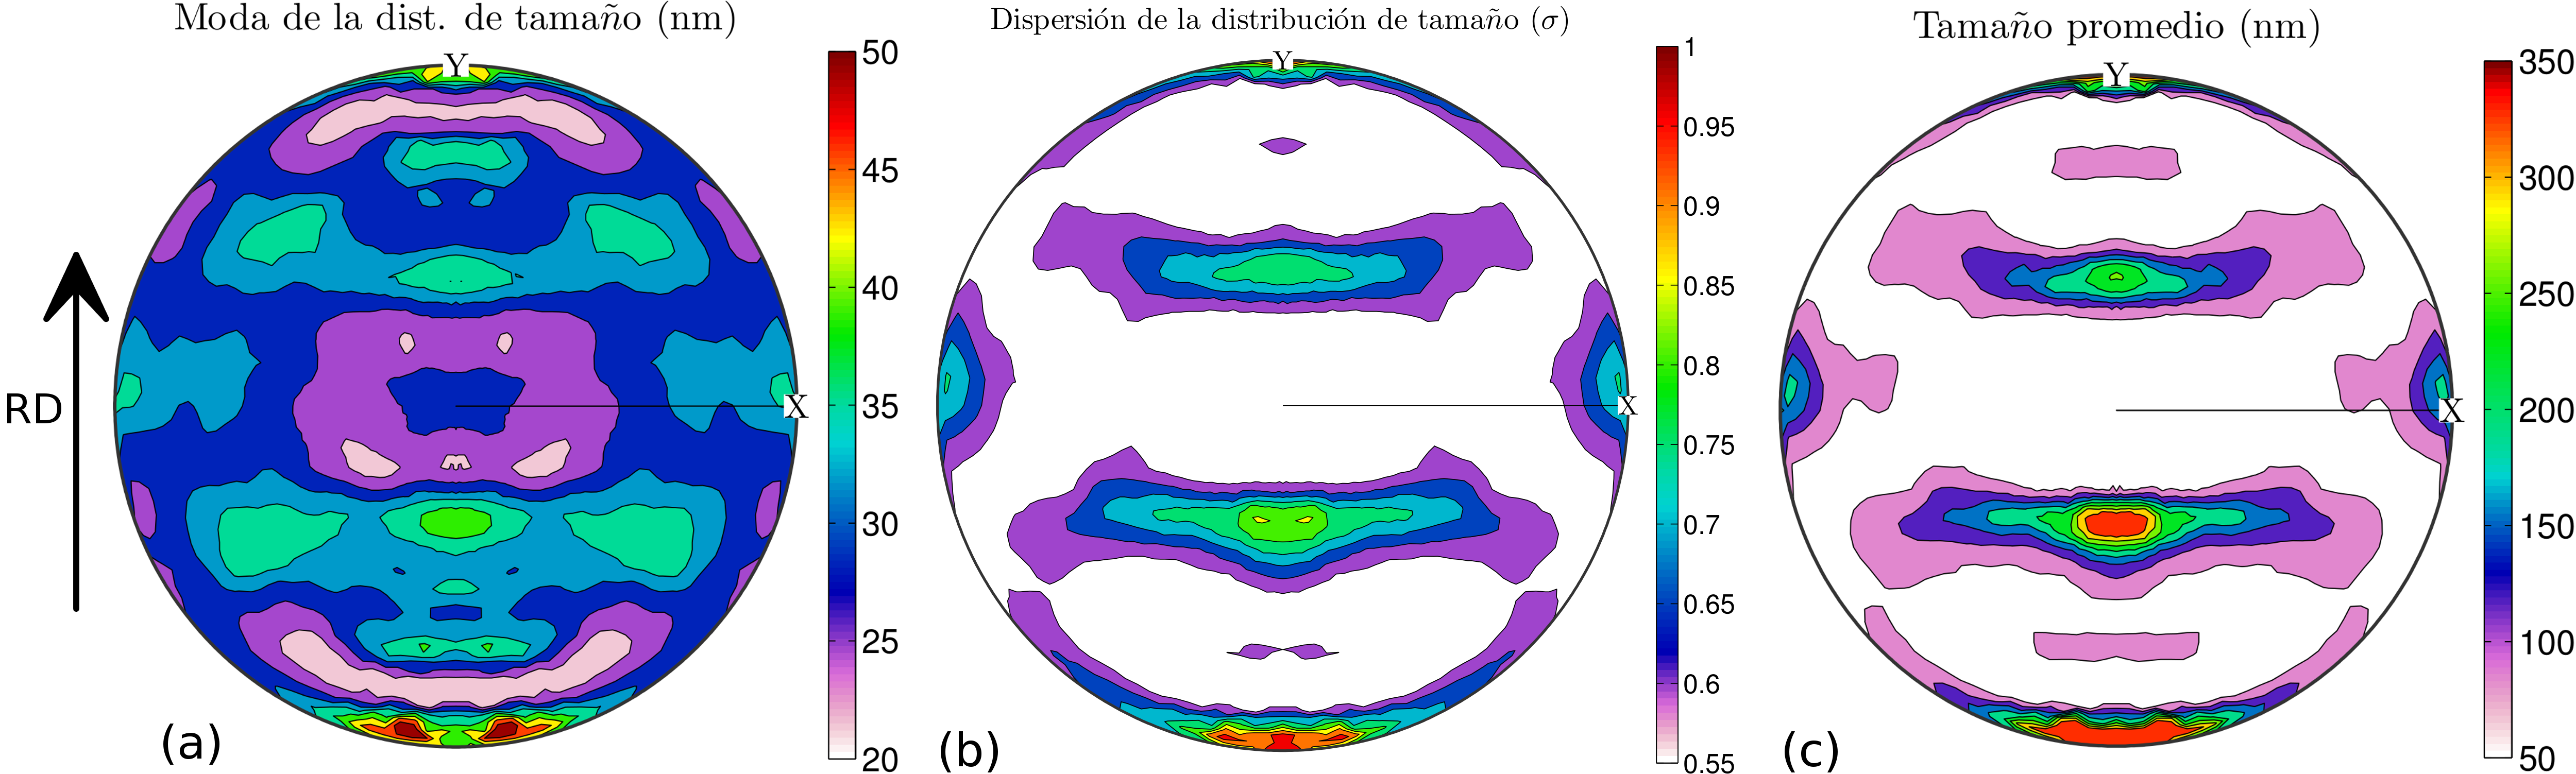
\includegraphics[width=\textwidth]{CMWP_size}
  \caption{Figuras de polos de la moda de la distribución lognormal de tamaño de cristalita (a), dispersión de dicha distribución (b) y tamaño medio de cristalita(c).}
  \label{fig:IFCMWPsize}
\end{figure}

\begin{figure}[!htb]
  \centering
  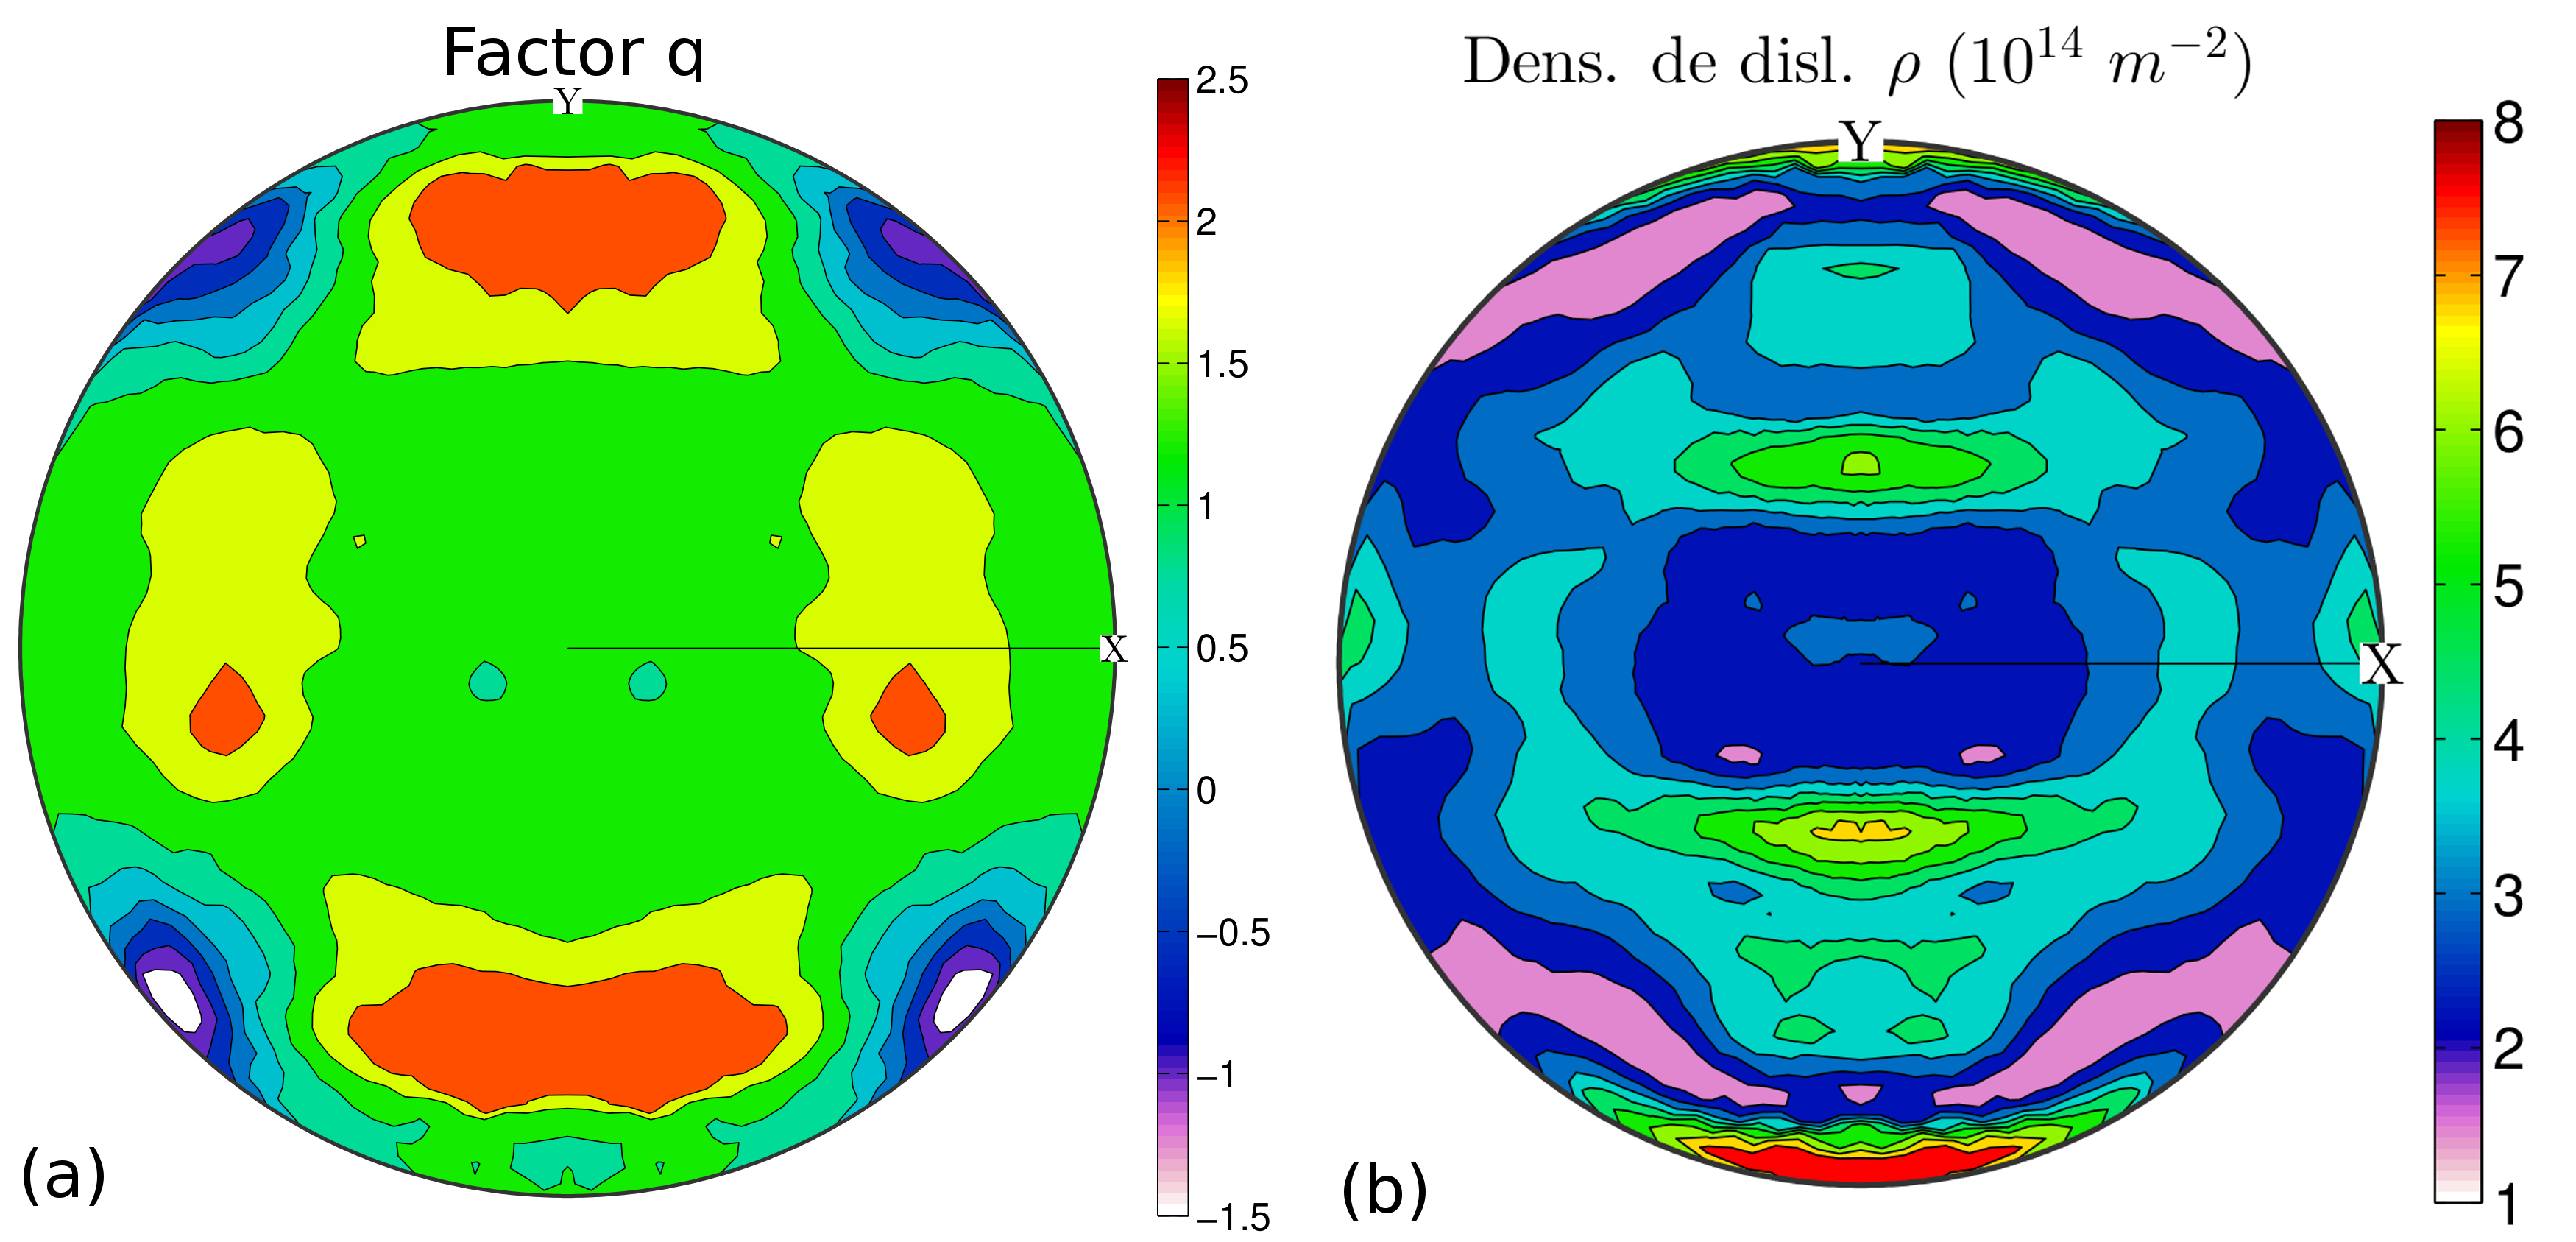
\includegraphics[width=0.7\textwidth]{CMWP_rho}
  \caption{(a) Figura de polo generalizadas del factor $q$ (según Ec. \ref{eq:Cav2}). (b) Figura de polos de densidad de dislocaciones.}
  \label{fig:IFCMWPrho}
\end{figure}

\begin{figure}[!htb]
  \centering
  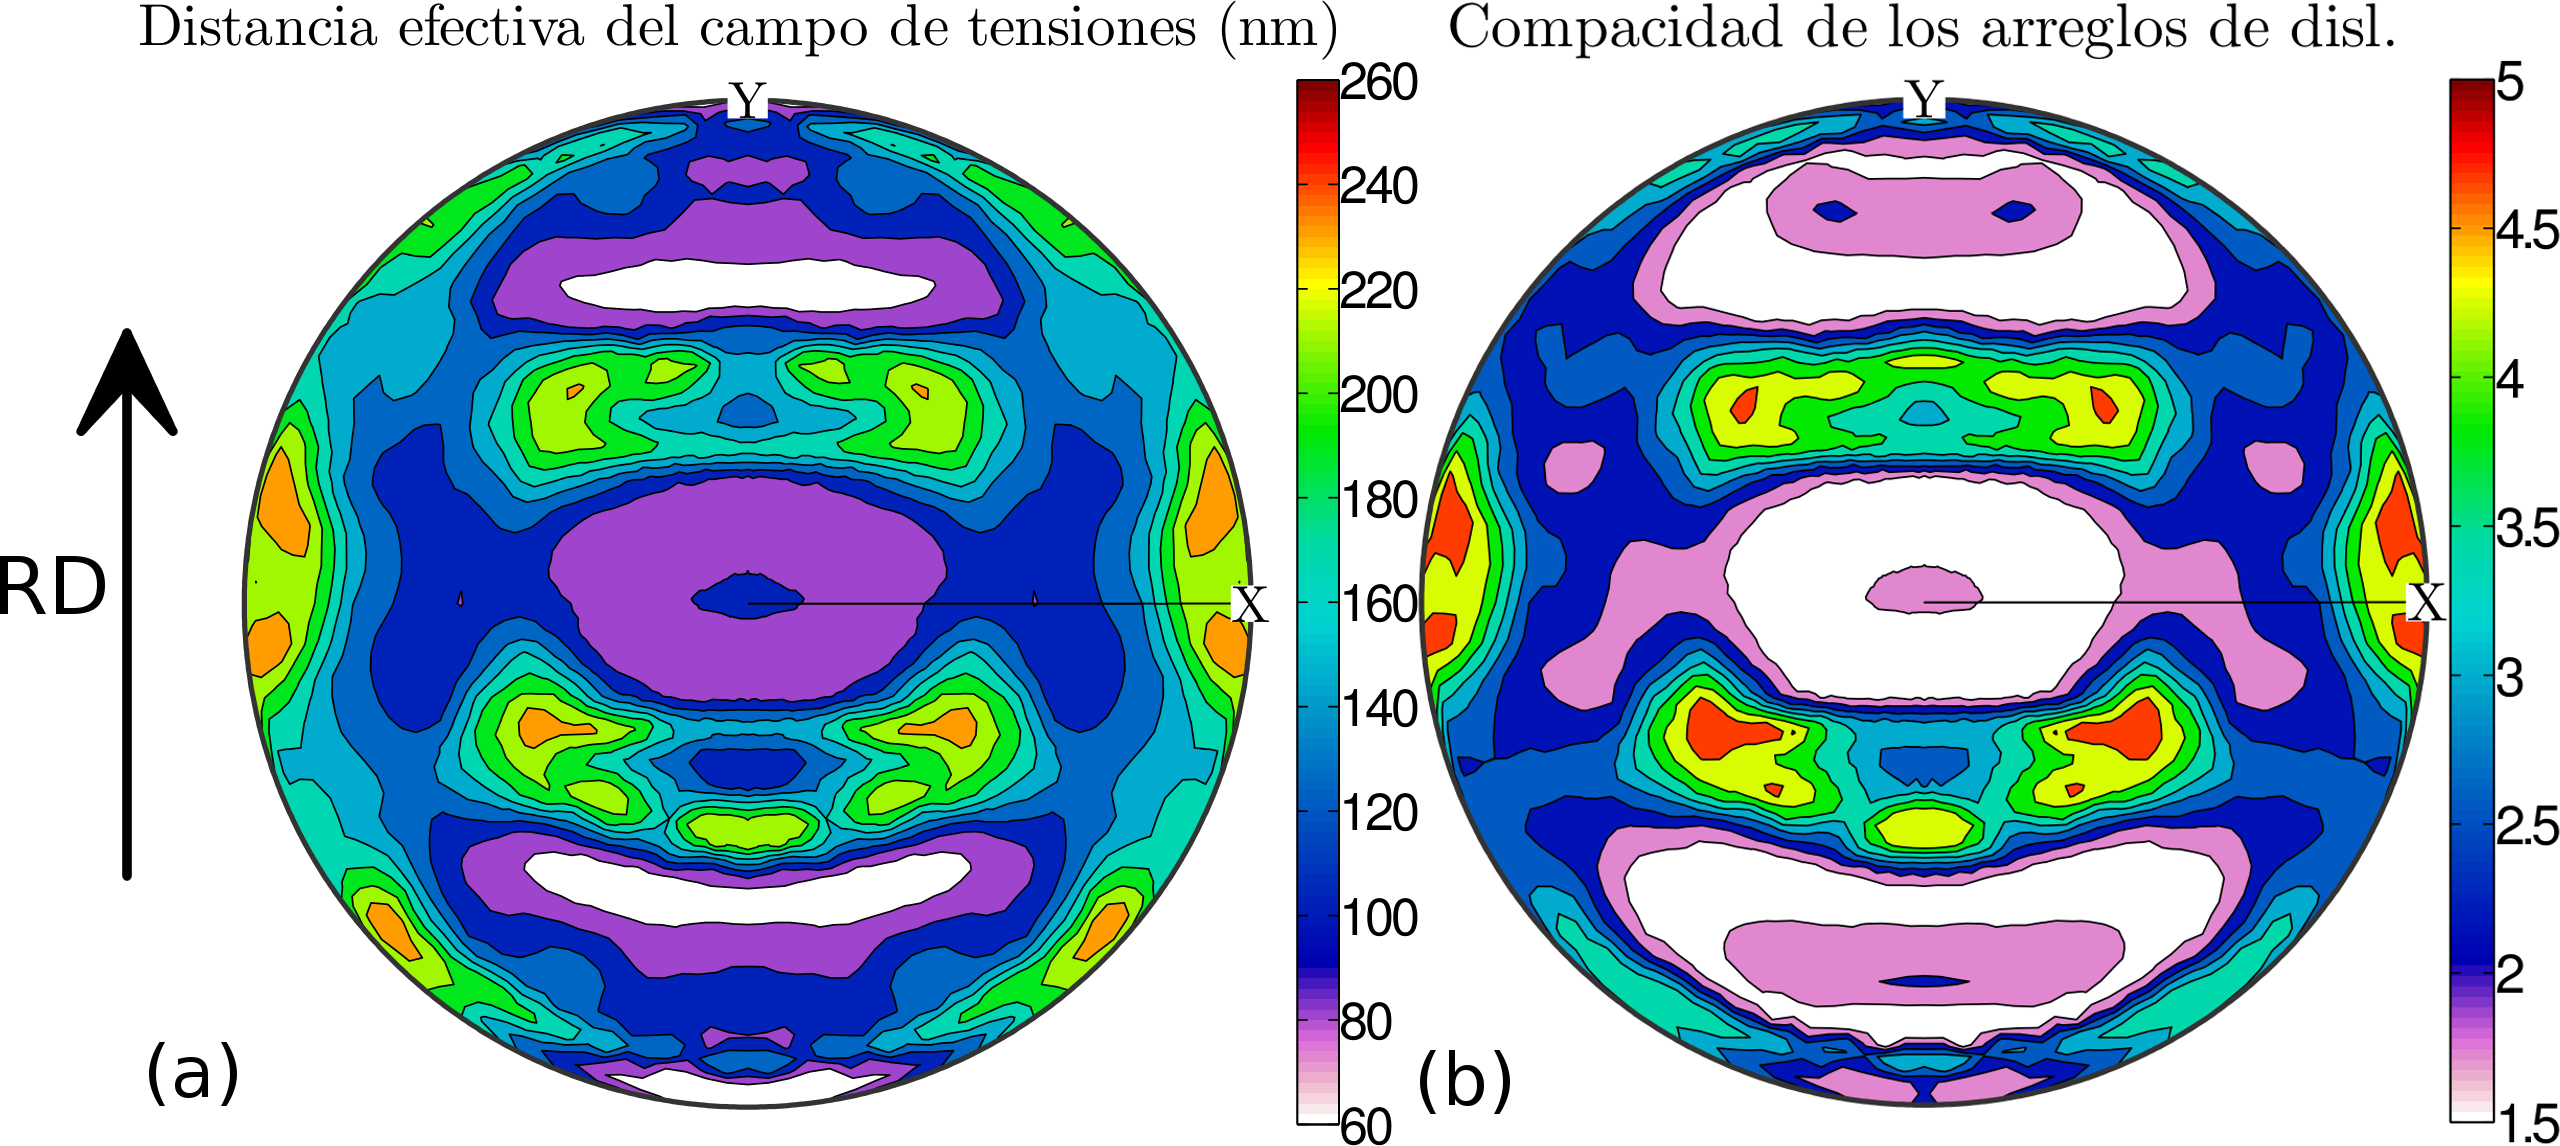
\includegraphics[width=0.7\textwidth]{CMWP_Re}
  \caption{Figuras de polos de (a) distancia del campo de distorsión producido por las dislocaciones y (b) Factor de Wilkens, indicador de la compacidad de los arreglos de dislocaciones.}
  \label{fig:IFCMWPRe}
\end{figure}

\newpage
\section{Estudio de la microestructura por EBSD}\label{S:IFEBSD}

\begin{figure}[!htb]
  \centering
  \includegraphics[width=\textwidth]{EBSD/IFEBSD}
  \caption{Mapa EBSD de figura de polo inversa EBSD del acero IF. La dirección de laminado RD es horizontal y la dirección normal a la chapa ND es hacia arriba. Puede verse como los granos tienen una forma ``alargada'' paralela con RD.}
  \label{fig:IFEBSD}
\end{figure}

\begin{figure}[!htb]
  \centering
  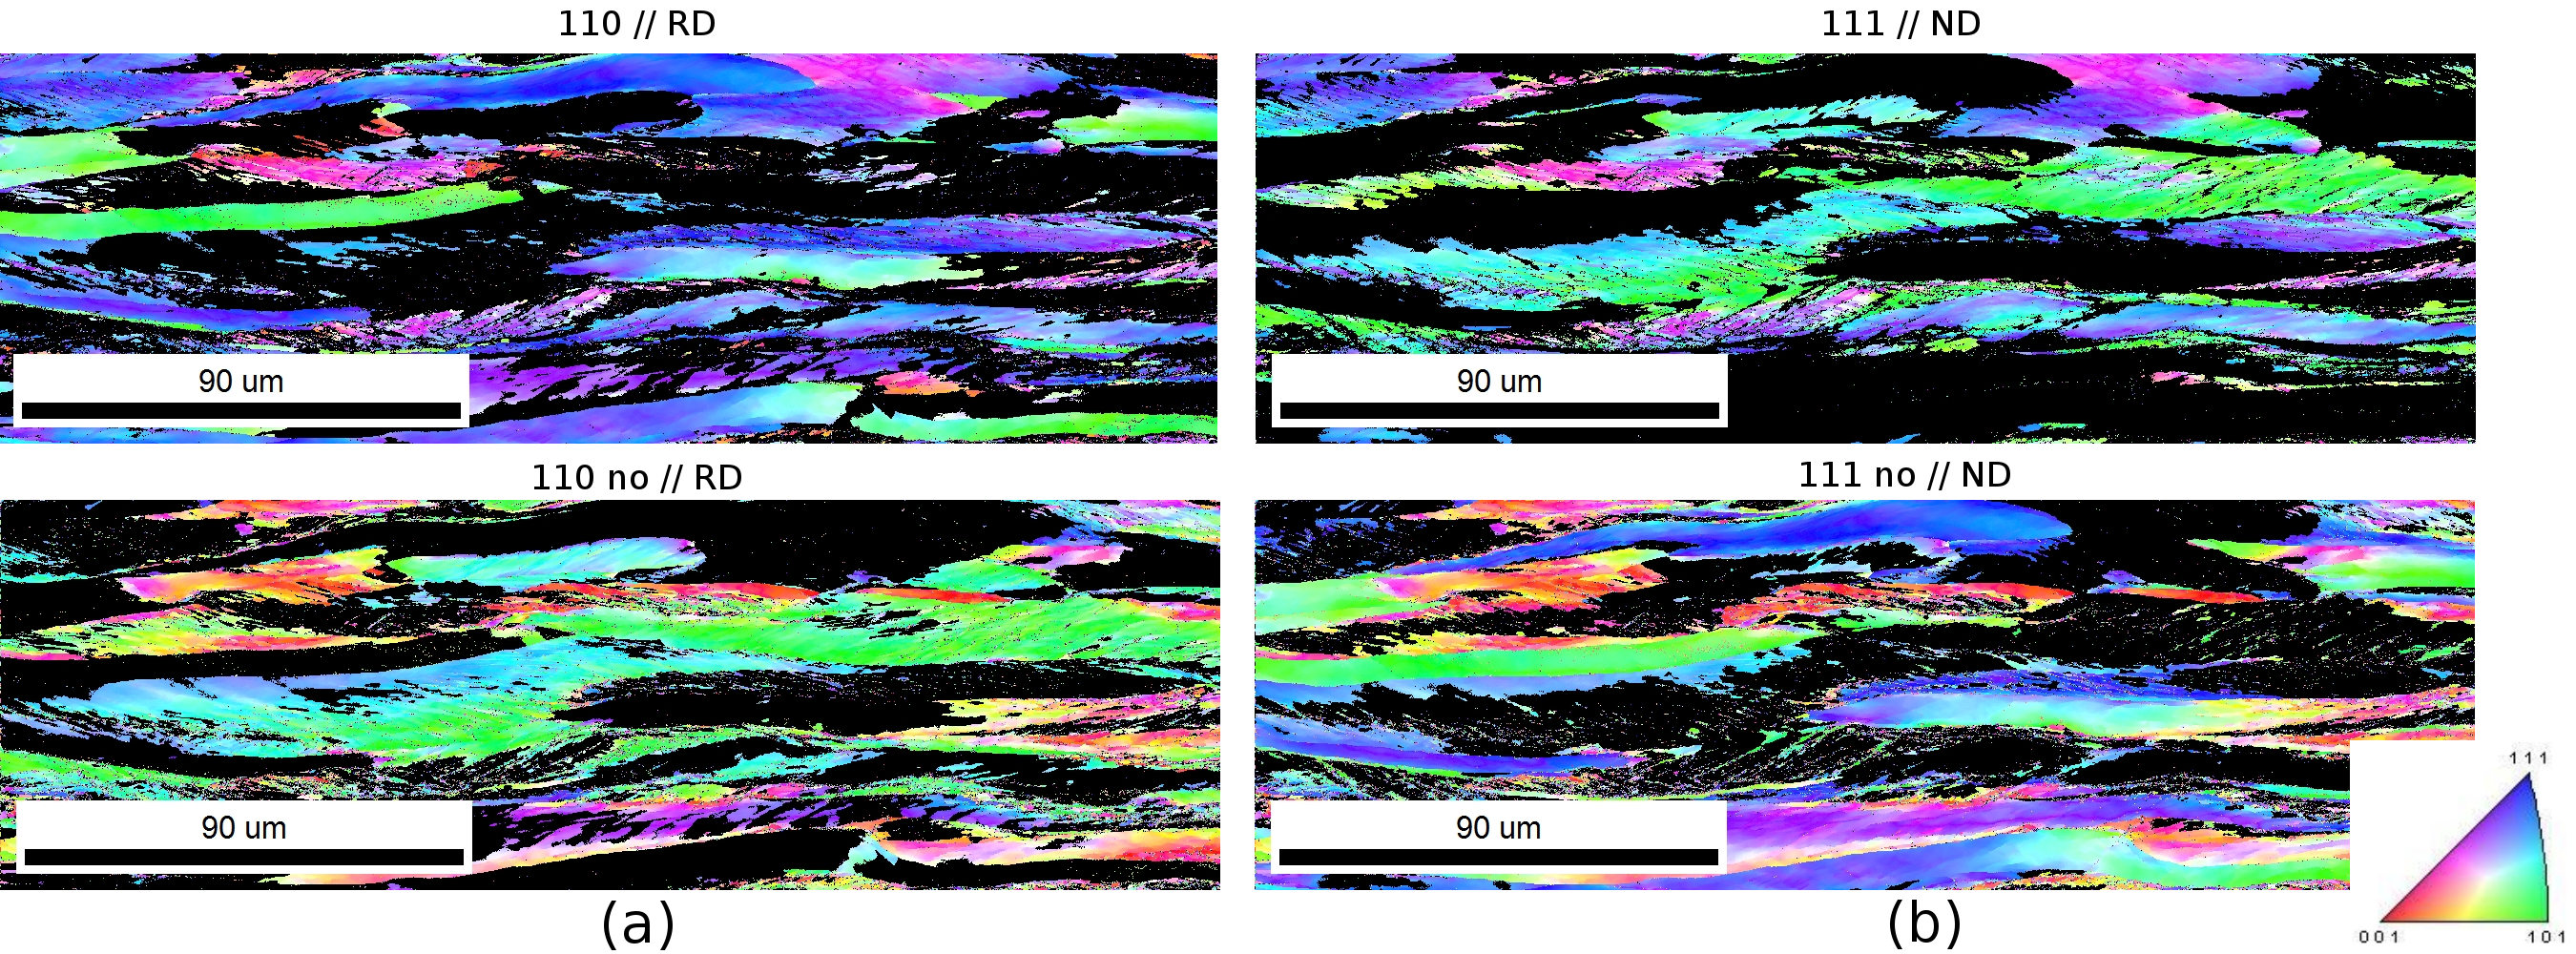
\includegraphics[width=\textwidth]{EBSD/IFEBSD_Partitions}
  \caption{Para estudiar la anisotropía en la microestructura del acero IF se tomaron los mapas de EBSD y se comparó la microestructura de las orientaciones cuyos planos $\{110\}$ eran perpendiculares a RD (pertenecientes a la fibra $\alpha$ y las que no. Se hizo la misma comparación con las orientaciones del mismo mapa que tenían sus planos $\{111\}$ perpendiculares a ND (pertenecientes a la fibra $\gamma$) y las que no lo tenían.}
  \label{fig:IFEBSDPar}
\end{figure}

\begin{figure}[!htb]
  \centering
  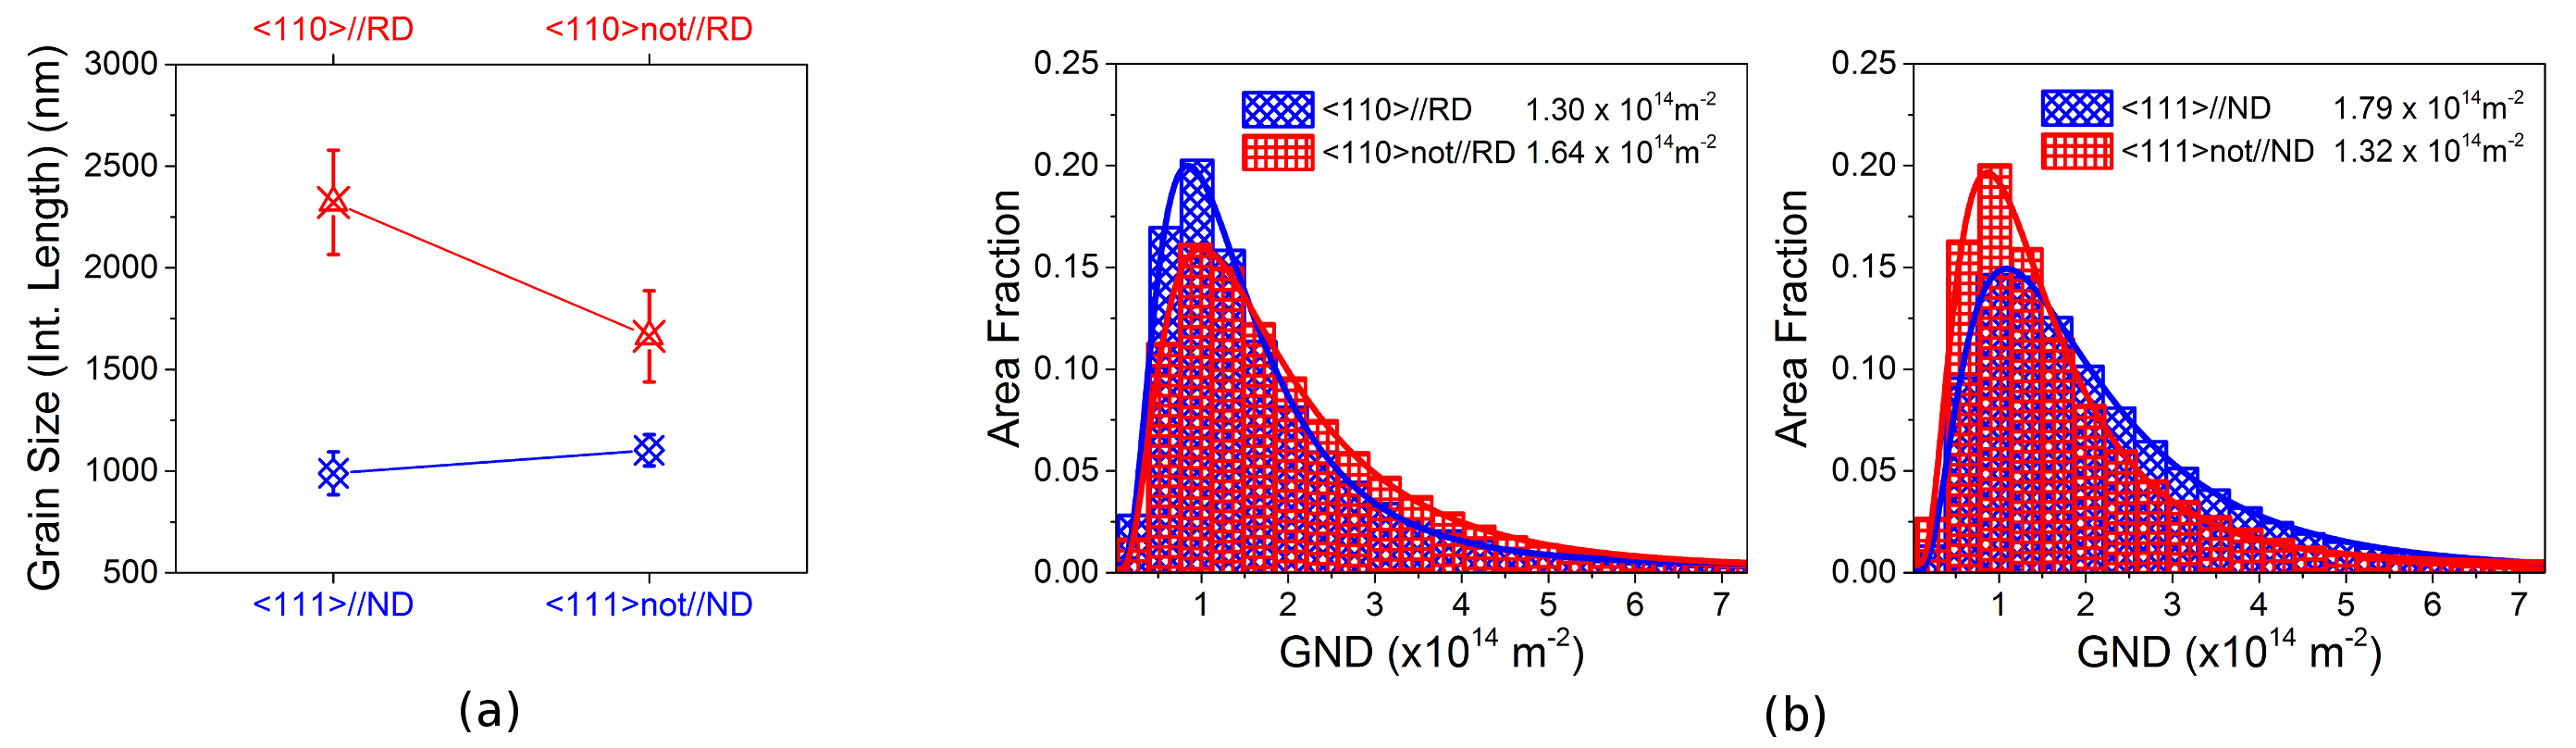
\includegraphics[width=\textwidth]{EBSD/IFEBSD_Size_GND}
  \caption{(a) Comparación del tamaño promedio de granos, medido según el método de longitud de intercepciones para las particiones de la Fig. \ref{fig:IFEBSDPar}. (b) Comparación de las dislocaciones geométricamente necesarias (GND) acumuladas en las particiones creadas.}
  \label{fig:IFEBSDVs}
\end{figure}

\newpage
\section{Discusión de resultados}\label{S:IFDis}
\section{Conclusiones}\label{S:IFConclusiones}
